%!TEX program = lualatex
% Arquivo: Template_Estat_Texto.tex

\documentclass[a4paper,12pt]{article}

% =========================================================
% Idioma e tipografia (LuaLaTeX)
% =========================================================
\usepackage[portuguese]{babel}
\usepackage{fontspec}
\setmainfont{Latin Modern Roman}

% =========================================================
% Layout
% =========================================================
\usepackage[top=3cm,bottom=2.5cm,left=3cm,right=2.5cm]{geometry}
\usepackage{setspace}
\onehalfspacing
\usepackage{indentfirst}
\setlength{\parindent}{1.25cm}

% =========================================================
% Matemática (align*, etc.)
% =========================================================
\usepackage{amsmath}
\usepackage{amssymb}

% =========================================================
% Tabelas, listas, figuras
% =========================================================
\usepackage{float}     % para [H]
\usepackage{booktabs}  % para \toprule, \midrule e \bottomrule
\usepackage{multirow}  % para \multirow
\usepackage{siunitx}   % para S, \si, \volt, \milli e \ampere

\sisetup{
    output-decimal-marker={,}
}
\usepackage{array}
\usepackage{enumitem}
\setlist[itemize]{noitemsep,topsep=3pt}
\setlist[enumerate]{noitemsep,topsep=3pt}

\usepackage{graphicx}
\usepackage{float}
\usepackage{pdflscape}
\graphicspath{{./}{./imagens/}{./figuras/}}

% =========================================================
% Links
% =========================================================
\usepackage{hyperref}
\usepackage{xurl}
\hypersetup{
  colorlinks=true,
  linkcolor=black,
  urlcolor=blue,
  citecolor=black,
  pdfauthor={},
  pdftitle={}
}
\sisetup{
    output-decimal-marker={,},
    table-number-alignment=center}
% =========================================================
% Dados da capa
% =========================================================
\newcommand{\Instituicao}{Universidade do Estado do Rio de Janeiro}
\newcommand{\Curso}{Física VI -- Oceanografia}
\newcommand{\Professor}{Professor: Alexandre Magnus Gomes Carvalho}
\newcommand{\Aluno}{Alunos: José Mauro Elsas}
\newcommand{\Cidade}{Rio de Janeiro}
\newcommand{\Ano}{2026}

\title{\textbf{Título do Documento}}
\author{\Aluno}
\date{\Cidade --- \Ano}

\begin{document}

% =========================================================
% Capa (página de rosto)
% =========================================================
\begin{titlepage}
\centering
{\large \Instituicao \par}
\vspace{0.5cm}
{\large \Curso \par}
\vspace{1.0cm}

{\LARGE \textbf{Experimento 1} \par}
\vspace{0.6cm}
{\Large Medidas Elétricas \par}

\begin{figure}[H]
  \centering
  
\includegraphics[width=.3\linewidth]{./uerj.jpg}
\end{figure}

\vfill

\begin{flushright}
\Aluno\\
\Professor
\end{flushright}

\vspace{1.0cm}
{\Cidade --- \Ano \par}
\end{titlepage}


% =========================================================
% Corpo do texto (exemplos)
% =========================================================
\section{Objetivos}

São os seguintes os objetivos desse relatório:

\begin{enumerate}[label=\alph*.]
  \item Determinar os desvios padrões das medições da fonte elétrica,
  tanto em tensão contínua quanto alternada;

  \item Determinar os desvios padrões dos valores medidos das resistências
  e verificar se o valor verdadeiro de cada resistência está no intervalo de
  medição.
\end{enumerate}

\section{Introdução}

O estudo da eletricidade desenvolveu-se a partir da observação de fenômenos naturais e de experimentos realizados ao longo de vários séculos. Embora manifestações elétricas já fossem conhecidas desde a Antiguidade, foi principalmente entre os séculos XVIII e XIX que a eletricidade passou a ser investigada de maneira sistemática. Os trabalhos de pesquisadores como Alessandro Volta, Georg Simon Ohm e Michael Faraday contribuíram para a compreensão das grandezas elétricas e para estabelecer relações quantitativas entre tensão, corrente e resistência. Esse desenvolvimento também levou à criação e ao aperfeiçoamento dos instrumentos destinados à medição dessas grandezas.

Com o avanço da instrumentação elétrica, tornou-se necessário avaliar não apenas o valor indicado por um aparelho, mas também a qualidade e a confiabilidade da medição realizada. Nenhuma medição experimental é absolutamente exata, pois seus resultados podem ser influenciados pela resolução e calibração dos instrumentos, pelas condições ambientais, pelas características do circuito e pelo próprio procedimento adotado. Assim, medições repetidas de uma mesma grandeza podem apresentar pequenas diferenças, formando um conjunto de valores distribuídos em torno de um valor médio.

A análise estatística permite descrever essa dispersão e avaliar a repetibilidade dos resultados. A média aritmética representa uma estimativa do valor central das medições, enquanto o desvio-padrão indica quanto os valores medidos se afastam, em geral, dessa média. Quanto menor for o desvio-padrão, menor será a dispersão entre as medições e maior será sua precisão. Entretanto, uma pequena dispersão não garante, isoladamente, a exatidão do resultado, pois as medições podem estar concentradas em torno de um valor diferente do valor verdadeiro ou de referência devido à presença de erros sistemáticos.

No caso de uma fonte elétrica, as medições de tensão contínua e de tensão alternada devem ser analisadas separadamente, uma vez que correspondem a diferentes modos de funcionamento e de leitura do instrumento. Para as resistências elétricas, além da determinação da média e do desvio-padrão das medições, pode-se construir um intervalo representativo da variação experimental e verificar se o valor de referência de cada resistor está contido nesse intervalo. Dessa forma, os fundamentos teóricos da média, do desvio-padrão, da precisão, da exatidão e do intervalo de medição fornecem a base necessária para atingir os objetivos deste experimento: avaliar a dispersão das medições da fonte elétrica e das resistências e comparar os resultados experimentais com os respectivos valores de referência.

\section{Materiais e Métodos}

Nesse Experimento foram usados os seguintes materiais:

\begin{enumerate}[label=\alph*.]

    \item Multímetro Digital com as suas devidas pontas de prova;

        \begin{figure}[H]
            \centering
            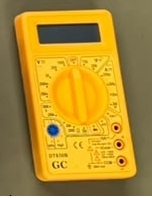
\includegraphics[width = 0.5\linewidth]{./Figs/digital.jpg}
            \caption{Multímetro Digital}
        \end{figure}

    \item Fonte de alimentação CA/CC estabilizada.

        \begin{figure}[H]
            \centering
            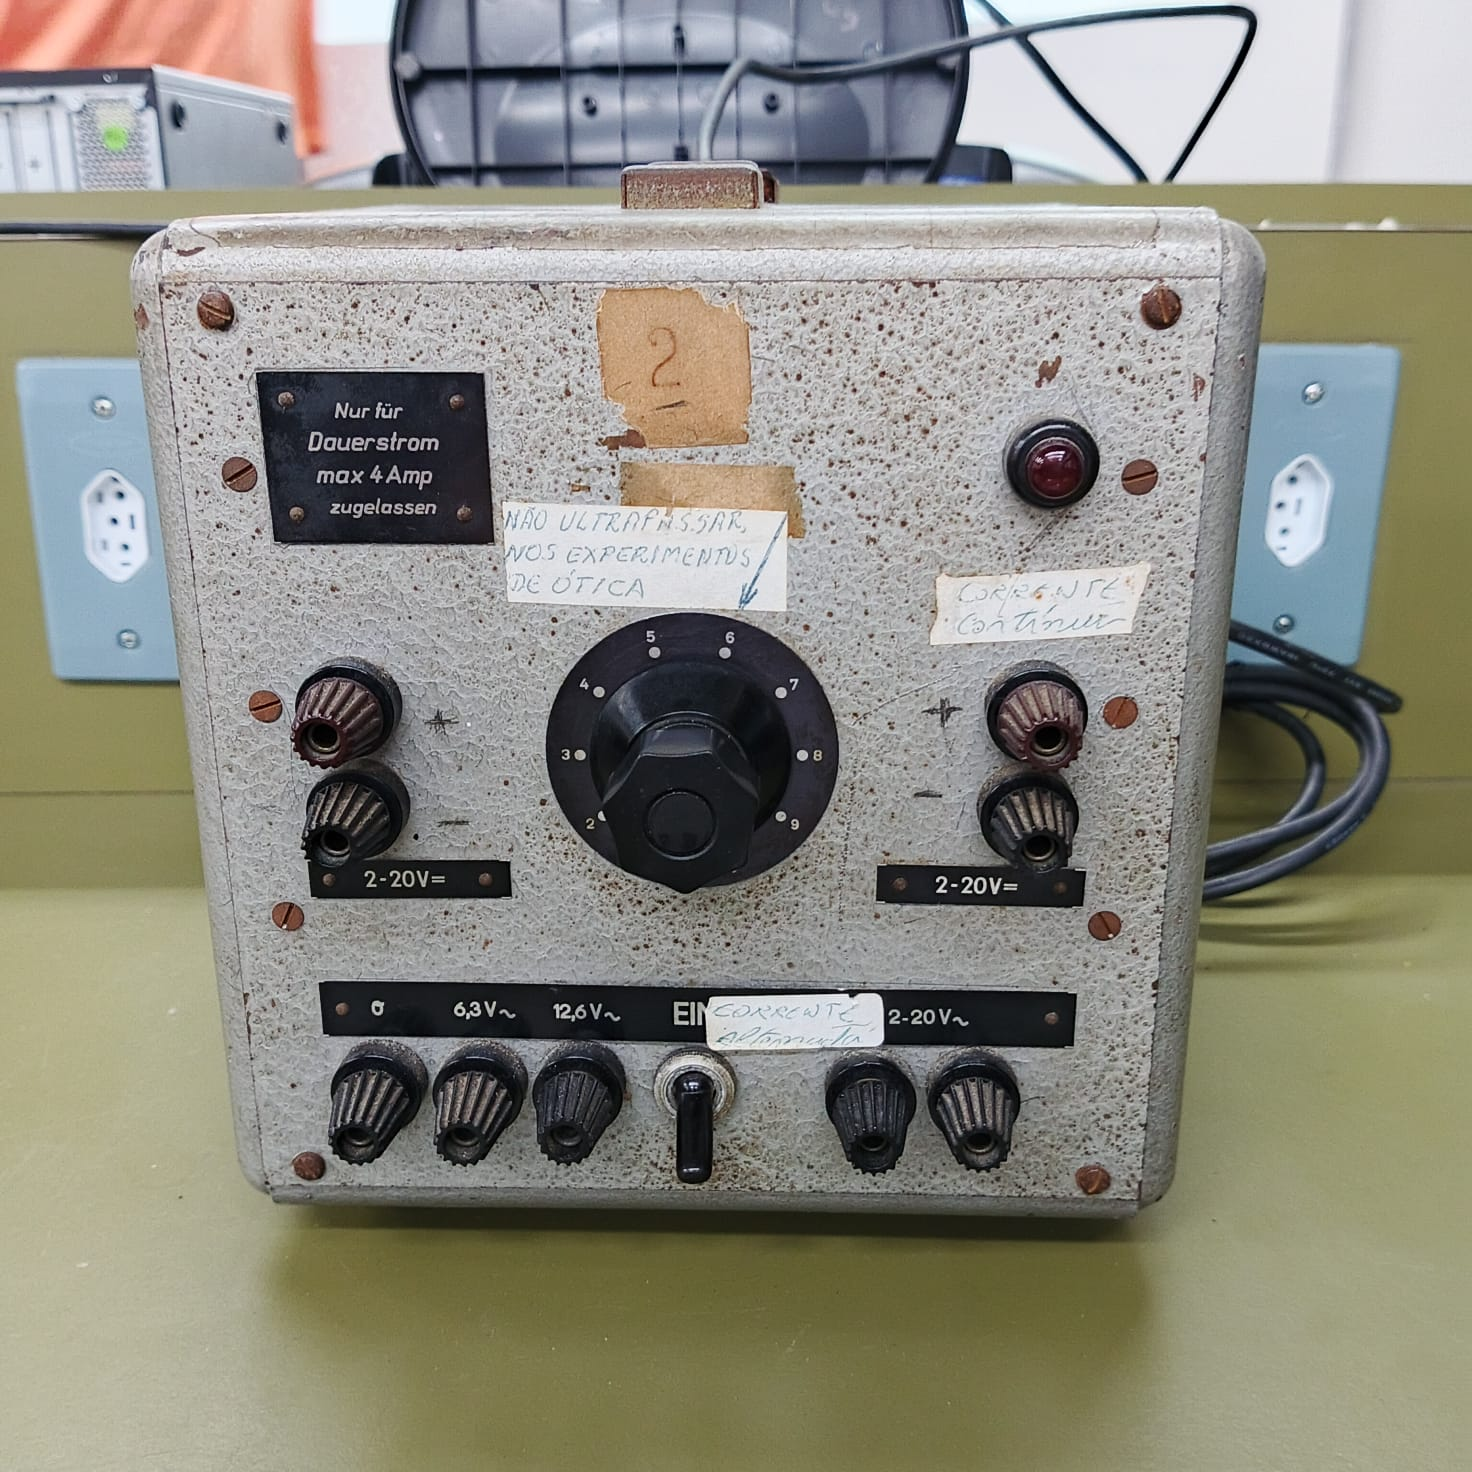
\includegraphics[width = .5\linewidth]{./Figs/fonte.jpeg}
            \caption{Fonte de alimentação}
        \end{figure}

    \item \textit{Protoboard} que é uma placa de ensaio  é uma base de plástico com furos e conexões internas condutoras, usada para montar e testar circuitos eletrônicos de forma rápida e temporária. Sua principal vantagem é dispensar o uso de solda, permitindo encaixar, remover e alterar componentes com facilidade.

    {https://ipelab.ufg.br/n/156373-protoboard-o-que-e-e-como-usar}

            \begin{figure}[H]
            \centering
            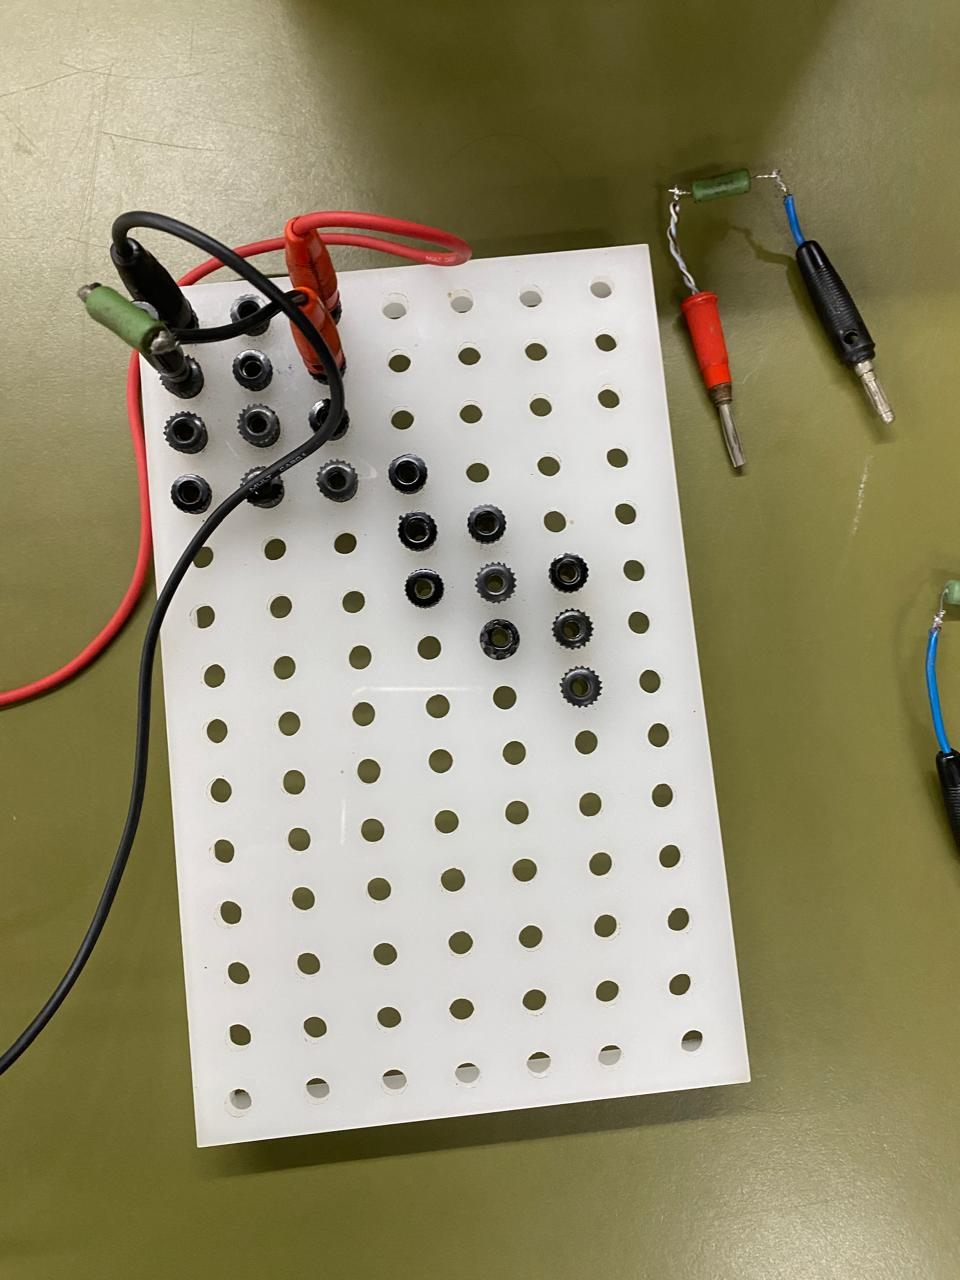
\includegraphics[width = .5\linewidth]{./Figs/protoboard.jpeg}
            \caption{\textit{Protoboard}}
        \end{figure}
    
    \item Resistores de diferentes valores.

          \begin{figure}[H]
            \centering
            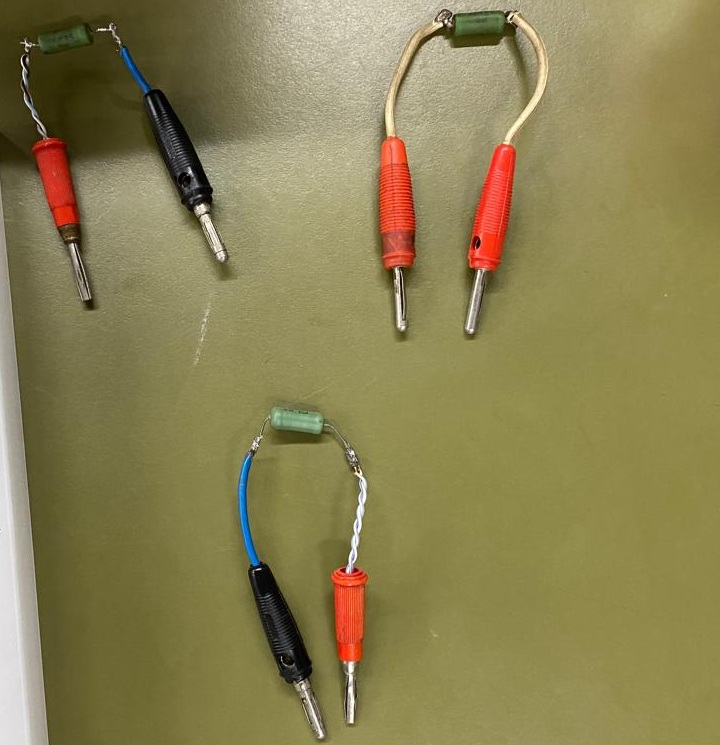
\includegraphics[width = .5\linewidth]{./Figs/resistores.jpeg}
            \caption{resistores de divers}
        \end{figure}

\section{Procedimento Experimental}

Para medir as tensões (Vcc e Vca), a fonte de alimentação foi conectada à rede elétrica e ligada, mantendo-se seus controles de tensão e corrente em condições adequadas para a realização das medições. 
Em seguida, o seletor de ajuste da fonte foi posicionado sucessivamente nas marcações 1, 4, 7, e 10.

Para cada uma dessas posições, foram feitas 5 medições da diferença de potencial fornecidos pela fonte configura para (Vcc e Vca). As medições de tensão foram realizadas com o voltímetro conectado em paralelo aos terminais de saída da fonte.

Usando o \textit{Protoboard} e as resistências foram feitas 

Em cada posição do seletor foram realizadas quatro medições independentes de
tensão. Os valores obtidos foram registrados em uma tabela, permitindo avaliar a repetibilidade das medições e as possíveis variações associadas aos instrumentos e à fonte de alimentação. Para cada conjunto de quatro medições, calculou-se a média aritmética, dada por:

\[
\bar{x} = \frac{1}{n}\sum_{i=1}^{n}\,x_i
\]

em que xi representa cada valor medido e n = 4 corresponde ao número de 
medições realizadas em cada posição.

O desvio padrão amostral foi calculado por:

\[
  s = \sqrt{\frac{\sum_{i=1}^{n}(x_1-\bar{x})^2}{n-1}}
\]

em que s representa o desvio padrão das medições. Esse parâmetro foi utilizado
para avaliar a dispersão dos valores em torno da média e, consequentemente, a
estabilidade das leituras obtidas em cada posição da fonte. As expressões da média
aritmética e do desvio padrão amostral seguem as definições usuais para uma amostra
de medições (Heckert et al., 2002, seção 7.2.2).

Ao final, os valores resistência elétrica foram apresentados na forma

\[
    R = (\bar{R} - \sigma)\, \Omega
\]


\end{enumerate}

\begin{table}[H]
    \centering
    \caption{Valores de tensão observados nas diferentes posições da fonte.}
    \medskip
    \label{tab:medicoes}

    \begin{tabular}{
        c
        S[table-format=2.1]
        S[table-format=2.1]
    }
        \toprule
        \textbf{Posição}
        & {\textbf{Tensão Contínua} (\si{\volt})}
        & {\textbf{Tensão Alternada} (\si{\volt})} \\
        \midrule

        \multirow{4}{*}{1}
        & 2,7 & 2,0 \\
        & 2,6 & 2,0 \\
        & 2,6 & 2,0 \\
        & 2,6 & 2,0 \\
        & 2,6 & 2,0 \\
        \midrule

        \multirow{4}{*}{4}
        & 11,5  & 8,5 \\
        & 11,5  & 8,6 \\
        & 11,5  & 8,6\\
        & 11,5  & 8,6\\
        & 11,5  & 8,6\\

        \midrule

        \multirow{4}{*}{7}
        & 20,5  & 14,8\\
        & 20,5  & 14,8\\
        & 20,5  & 14,8\\
        & 20,5  & 14,8\\
        & 20,5  & 14,8\\
        \midrule

        \multirow{4}{*}{10}
        & 29,5  & 21,4\\
        & 29,5  & 21,4\\
        & 29,5  & 21,4\\
        & 29,5  & 21,4\\
        & 29,5  & 21,3\\
        \bottomrule
    \end{tabular}
\end{table}

\subsection{Médias das leituras de Tensão}

\begin{table}[H]
    \centering
    \caption{Valores nominais e medidos das resistências elétricas.}
    \label{tab:resistores_medidos}
    \medskip

\begin{table}[H]
    \centering
    \caption{Valores médios das tensões contínua e alternada.}
    \label{tab:medias_vcc_vca}
    \medskip

    \begin{tabular}{ccc}
        \toprule
        \textbf{Posição}
        & \shortstack{\textbf{Média de \(V_{\mathrm{CC}}\)}\\(\si{\volt})}
        & \shortstack{\textbf{Média de \(V_{\mathrm{CA}}\)}\\(\si{\volt})} \\
        \midrule
        1  & 2,62 & 2,00  \\
        4  & 11,5 & 8,58  \\
        7  & 20,5 & 14,8  \\
        10 & 29,5 & 21,38 \\
        \bottomrule
    \end{tabular}
\end{table}

\begin{figure}[H]
    \centering
    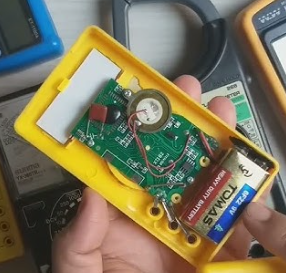
\includegraphics[width=0.65\linewidth]{./Figs/multimetro_bateria.png}
    \caption{Multímetro digital com bateria à vista.}
    \label{fig:multi_dig}

    \vspace{0.2cm}
    {\footnotesize Fonte: \url{https://www.youtube.com/watch?v=zhguLb29z2M}.}
\end{figure}

Assim, temos o gráfico \ref{graf:graf_comp}, que compara os valores nominais e os valores medidos.

\begin{figure}[H]
    \centering
    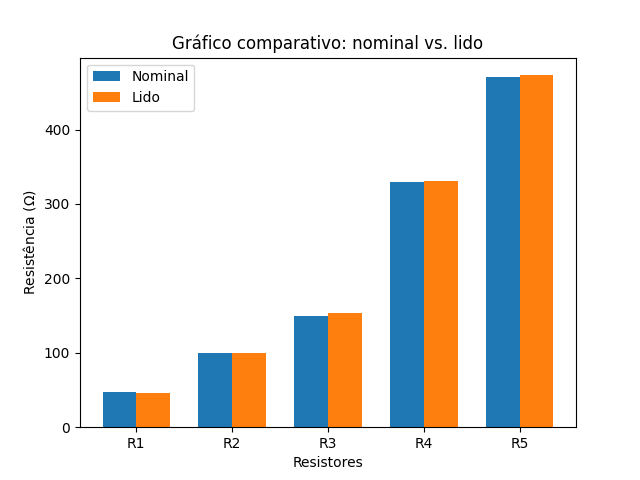
\includegraphics[width=0.8\linewidth]{./Figs/graf_cpmparativo.png}
    \caption{Comparação entre os valores nominais e os valores medidos das resistências.}
    \label{graf:graf_comp}
\end{figure}

\begin{itemize}
    \item Calcule a diferença percentual, usando a expressão abaixo, entre os valores medidos com o multímetro e os valores nominais do fabricante. Considerando que os resistores utilizados possuem tolerância de até 5\%, as medidas realizadas estão dentro da tolerância especificada pelo fabricante.
    
    Para calcular o erro $\epsilon\%$ foi usada a fórmula:

    \[
        \epsilon\%=\frac{|R_{medido}-R_{nominal}|}{R_{nominal}}\times 100
    \]

\begin{figure}[H]
    \centering
    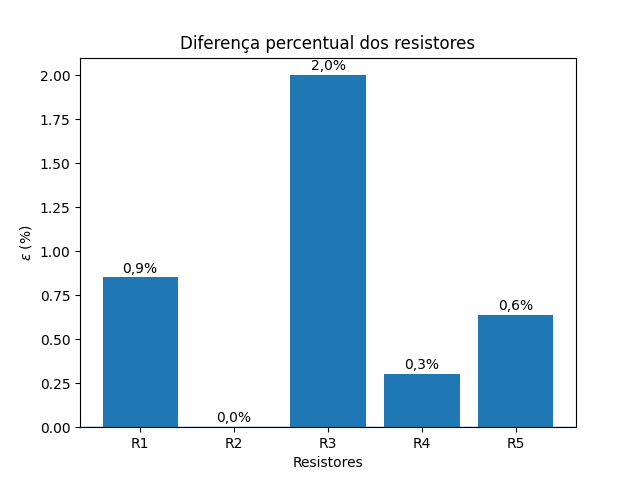
\includegraphics[width=0.8\linewidth]{./Figs/graf_cpmparativo_2.png}
    \caption{Diferença percentual entre os valores nominais e os valores medidos das resistências.}
    \label{graf:diferenca_percentual}
\end{figure}
\end{itemize}

\end{document}